\documentclass[12pt]{article}
\usepackage{fullpage}
\usepackage{lscape}
\usepackage[top=2cm, bottom=4.5cm, left=2.5cm, right=2.5cm]{geometry}
\usepackage{amsmath,amsthm,amsfonts,amssymb,amscd}
\usepackage{lastpage}
\usepackage{enumerate}
\usepackage{fancyhdr}
\usepackage{mathrsfs}
\usepackage{graphicx}
\usepackage{subcaption}
\usepackage{listings}
\usepackage{hyperref}
\usepackage{titlesec}
\usepackage[T1]{fontenc}
\usepackage[utf8]{inputenc}
\usepackage{palatino}
\usepackage{booktabs}
\usepackage[dvipsnames]{xcolor}
\usepackage{enumitem}
\usepackage{bm}

\definecolor{grey}{gray}{0.6}
\lstset{
    escapeinside={(*@}{@*)},
}

\newcommand{\SubItem}[1]{
    {\setlength\itemindent{15pt} \item[-] #1}
}

\newcommand\twoitems[2]{%
\item#1%
\hspace{20pt}%
\labelitemi
\hspace{\labelsep}#2
}

\setcounter{secnumdepth}{4}
\titleformat{\paragraph}
{\normalfont\normalsize\bfseries}{\theparagraph}{1em}{}
\titlespacing*{\paragraph}
{0pt}{3.25ex plus 1ex minus .2ex}{1.5ex plus .2ex}

\hypersetup{%
  colorlinks=true,
  linkcolor=blue,
  linkbordercolor={0 0 1}
}

\lstdefinestyle{C++}{
    language        = C,
    frame           = lines, 
    basicstyle      = \footnotesize\ttfamily,
    keywordstyle    = \color{blue},
    stringstyle     = \color{olive},
    commentstyle    = \color{red}\ttfamily,
    breaklines      = true,
    tabsize         = 2
}

\setlength{\parindent}{0.0in}
\setlength{\parskip}{0.05in}

\newcommand\code{\texttt}
\newcommand\course{COMP0017}
\newcommand\hwnumber{}                   
\pagestyle{fancyplain}
\headheight 35pt
\lhead{\NetIDa}
\lhead{\course}                 
\chead{\textbf{\Large Assessment \hwnumber}}
\rhead{\today}
\lfoot{}
\cfoot{}
\rfoot{\small\thepage}
\headsep 1.5em

\graphicspath{{./imgs/}}

\renewcommand{\thesubsection}{\thesection.\alph{subsection}}
\renewcommand{\thesubsubsection}{\thesubsection.\roman{subsubsection}}

\begin{document}

\section{}

\subsection{}

Assuming the tape structure below ($c_i \in \Sigma$):
$$
\triangleright \;|\; \sqcup\;(\leftarrow q_0) \;|\; c_0 \;|\; c_1 \;|\; ... \;|\; c_n \;|\; \sqcup \;|\; ...
$$

We can design a TM where all undefined transitions leads to a rejection, and the halting state $h$ means accept:
$$ 
\begin{aligned}
M &= \{\Sigma_M, Q, q_0, H, \delta\} \\
\Sigma_M & = \{0, 1, \triangleright, \sqcup\} \\
Q & = \{q_0, q_1, h\} \\
H & = \{h\} \\
\delta\{q_0, \sqcup\} & = \{q_1, \rightarrow\} \\
\delta\{q_1, 0\} & = \{q_1, \rightarrow\} \\
\delta\{q_1, 1\} & = \{q_1, \rightarrow\} \\
\delta\{q_1, \sqcup\} &= \{h, \sqcup\}
\end{aligned}
$$

Note that this TM mentioned above also checks for tape structure correctness. We can further reduce the number of states to a TM with only one state $h$ (as both the initial and the halting state) with no transition, if we do not need to verify tape's correctness.

\subsection{}
\begin{itemize}
    \item $L_1$ is undecidable but recognisable, and Rice's theorem doesn't apply (behavioural property).
    \item $L_2$ is undecidable but recognisable, and Rice's theorem applies (nontrivial language property).
    \item $L_3$ is unrecognisable, and Rice's theorem applies (nontrivial language property).
    \item $L_4$ is decidable, and Rice's theorem doesn't apply (structural property).
\end{itemize}

\subsection{}
To prove $L_6 \leq_m L_5$, we construct a mapping function $f(y_6) = y_5$, as defined below:
\begin{itemize}
    \item If $y_6 \neq code(M)$ for all $M$, then $f(y_6) = y_6$
    \item If $y_6 = code(M_6)$, then $f(y_6) = code(M_5)$ where $M_5$ is constructed as follows:
    \SubItem{$M_5$ first reads the tape and compare it with $code(M_5)$}
    \SubItem{If the tape content is the same as $code(M_5)$, $M_5$ will clear the tape, write $010$, reset the tape head, and then simulate $M_6$}
    \SubItem{Otherwise, $M_5$ enters a loop}
\end{itemize}

To prove the reduction correctness, we consider the following three cases,
\begin{itemize}
    \item If $y_6 \notin L_6$ and $y_6 \neq code(M)$ for all $M$, $f(y_6) = y_6 \notin L_5$
    \item If $y_6 \notin L_6$ but $y_6 = code(M)$ for some TM $M$, $f(y_6) = code(M_5)$ which simulates $M$ on input $010$ (when read $code(M_5)$ on tape), and \textbf{does NOT halt} as $y_6 = code(M) \notin L_6$. When not reading $code(M_5)$ on tape, by definition, $M_5$ does not halt. Thus, $M_5$ does not halt in either case and $code(M_5) \notin L_5$
    \item If $y_6 = code(M_6) \in L_6$, $f(y_6) = code(M_5)$ which \textbf{does halt} (when read $code(M_5)$ on the tape) as simulating $code(M_6) \in L_6$ is said to halt on input $010$. Thus, $M_5$ halts on $code(M_5)$ and $code(M_5) \in L_5$
\end{itemize}

\subsection{}

\subsubsection{}
Given $L^-$ is unrecognisable, the statement "$L$ is never decidable" is \textbf{TRUE}.

If $L$ is decidable, there exists a TM $M$ that accepts string $s \in L$ and rejects $s \notin L$. We swap the accept and rejection states to create a $M^-$ which accepts $s \notin L$. Note that $s \notin L \iff s \in L^-$. Hence $M^-$ recognises $L^-$. There is a contradiction here.

Hence, we proved $L$ is never decidable.

\subsubsection{}
Given $L^-$ is unrecognisable, the statement "$L$ is never recognisable" is \textbf{FALSE}.

We show a counter example here. Let $L$ be a recognisable but undecidable language $HALT$, $L^- = HALT^-$ is not recognisable.

Furthermore, it is provable by contradiction that any recognisable but undecidable language $L_r$ will have an unrecognisable complement $L_r^-$. 

Assume $L_r^-$ is also recognisable, there exists two TMs $M$ and $M^-$ that recognises $L_r$ and $L_r^-$ respectively. We can combine the two TMs and construct a TM $M_d$ that has two tapes with the same input and simulates $M$ and $M^-$ in parallel. $M_d$ accepts if $M$ accepts and rejects when $M^-$ accepts. Thus, $L_r$ is now decidable, hence contradicts. 

Therefore, we proved that $L_r^-$ must be unrecognisable as a complement of a recognisable but undecidable language $L_r$.

With the above proof, $L$ can be any recognisable but undecidable language to make $L^-$ unrecognisable.

\section{}

\subsection{}
Assume the $\pmb{EXTIME}$ complexity class actually means $\pmb{EXPTIME}$ (a typo).

Given a decision problem $A$,

\begin{itemize}
    \item $A \in \pmb{NP}$ iff. there exists a non-deterministic TM $M$ that accepts all yes-instances of $A$ and rejects all no-instances of $A$ in run-time $O(n^k)$ for some fixed $k$ (in p-time).
    \item $A \in \pmb{PSPACE-complete}$ iff.
    \SubItem{$A \in \pmb{PSPACE}$, and} 
    \SubItem{for all $B \in \pmb{PSPACE}$, $B \leq_p A$}
    \item $A \in \pmb{NPSPACE-complete}$ iff.
    \SubItem{$A \in \pmb{NPSPACE}$, and} 
    \SubItem{for all $B \in \pmb{NPSPACE}$, $B \leq_p A$}
    \item $A \in \pmb{EXPTIME}$ iff. there exists a deterministic TM $M$ that accepts all yes-instances of $A$ and rejects all no-instances of $A$ in run-time $O(2^{p(n)})$ where $p(n)$ is a polynomial of $n$. 
\end{itemize}

Also, we append the definitions to complement the definitions of $\pmb{PSPACE-complete}$ and $\pmb{NPSPACE-complete}$
\begin{itemize}
    \item $A \in \pmb{PSPACE}$ iff. there is exists a deterministic TM $M$ that solves $A$, and if $M$ runs with an input instance $a$, and $|a| \leq n$, then only tape cells $0,1,2...\;p(n) - 1$ (where $p(n)$ is a polynomial of $n$) are ever accessed during the computation. 
    \item $A \in \pmb{NPSPACE}$ iff. there is exists a non-deterministic TM $M$ that solves $A$, and if $M$ runs with an input instance $a$, and $|a| \leq n$, then only tape cells $0,1,2...\;p(n) - 1$ (where $p(n)$ is a polynomial of $n$) are ever accessed during the computation. 
\end{itemize}

\subsection{}
\begin{itemize}
    \item $\pmb{NP} \subseteq \pmb{EXPSPACE}$
    \item $\pmb{PSPACE-complete} = \pmb{NPSPACE-complete} \subseteq \pmb{EXPSPACE}$
\end{itemize}

\subsection{}
Given any two problems $A, B \in \pmb{PSPACE-complete}$.

By definition,

$A \in \pmb{PSPACE-complete}$ means $A \in \pmb{PSPACE}$

$B \in \pmb{PSPACE-complete}$ means $\forall C \in \pmb{PSPACE}\; C \leq_p B $

Since $A \in \pmb{PSPACE}$, we show $ A \leq_p B $

Vice versa,

$B \in \pmb{PSPACE-complete}$ means $B \in \pmb{PSPACE}$

$A \in \pmb{PSPACE-complete}$ means $\forall C \in \pmb{PSPACE}\; C \leq_p A $

Thus, given $ B \in \pmb{PSPACE}$, we also show $B \leq_p A$

By definition, $A \leq_p B ,\; B \leq_p A$,  we conclude that $A \equiv_p B $

Therefore, for any two $\pmb{PSPACE-complete}$ problems, they are p-time equivalent to each other.

\subsection{}

\begin{enumerate}
    \item Yes-instance. $p$ can be $\top$.
    \item Yes-instance. When $p$ is $\top$, $q$ can be $\top$. When $p$ is $\bot$, $q$ can still be $\top$.
    \item Yes-instance. Let $p$ be $\bot$, no matter what $q$ is this instance evaluates to $\top$.
    \item No-instance. If $p$ is $\top$, $\forall q$ doesn't satisfy when $q$ is $\bot$. If $p$ is $\bot$, $\forall q$ still doesn't satisfy when $q$ is $\top$.
    \item No-instance. Say $q$ is $\top$, when $\forall p$ evaluates to $\top$, there would be no $r$ to satisfy this instance. Say $q$ is $\bot$, when $\forall p$ evaluates to $\bot$, $(p \lor q)$ would evaluate to $\bot$ and unsatisfy this instance.
    \item Yes-instance. When $p$ is $\top$, exist $q\; \bot$ and $r\; \top$ to satisfy this instance. When $p$ is $\bot$, exist $q \; \top$ and $r\; \bot$ to satisfy this instance.
\end{enumerate}

\subsection{}

\begin{figure}[h!]
  \makebox[\textwidth][c]{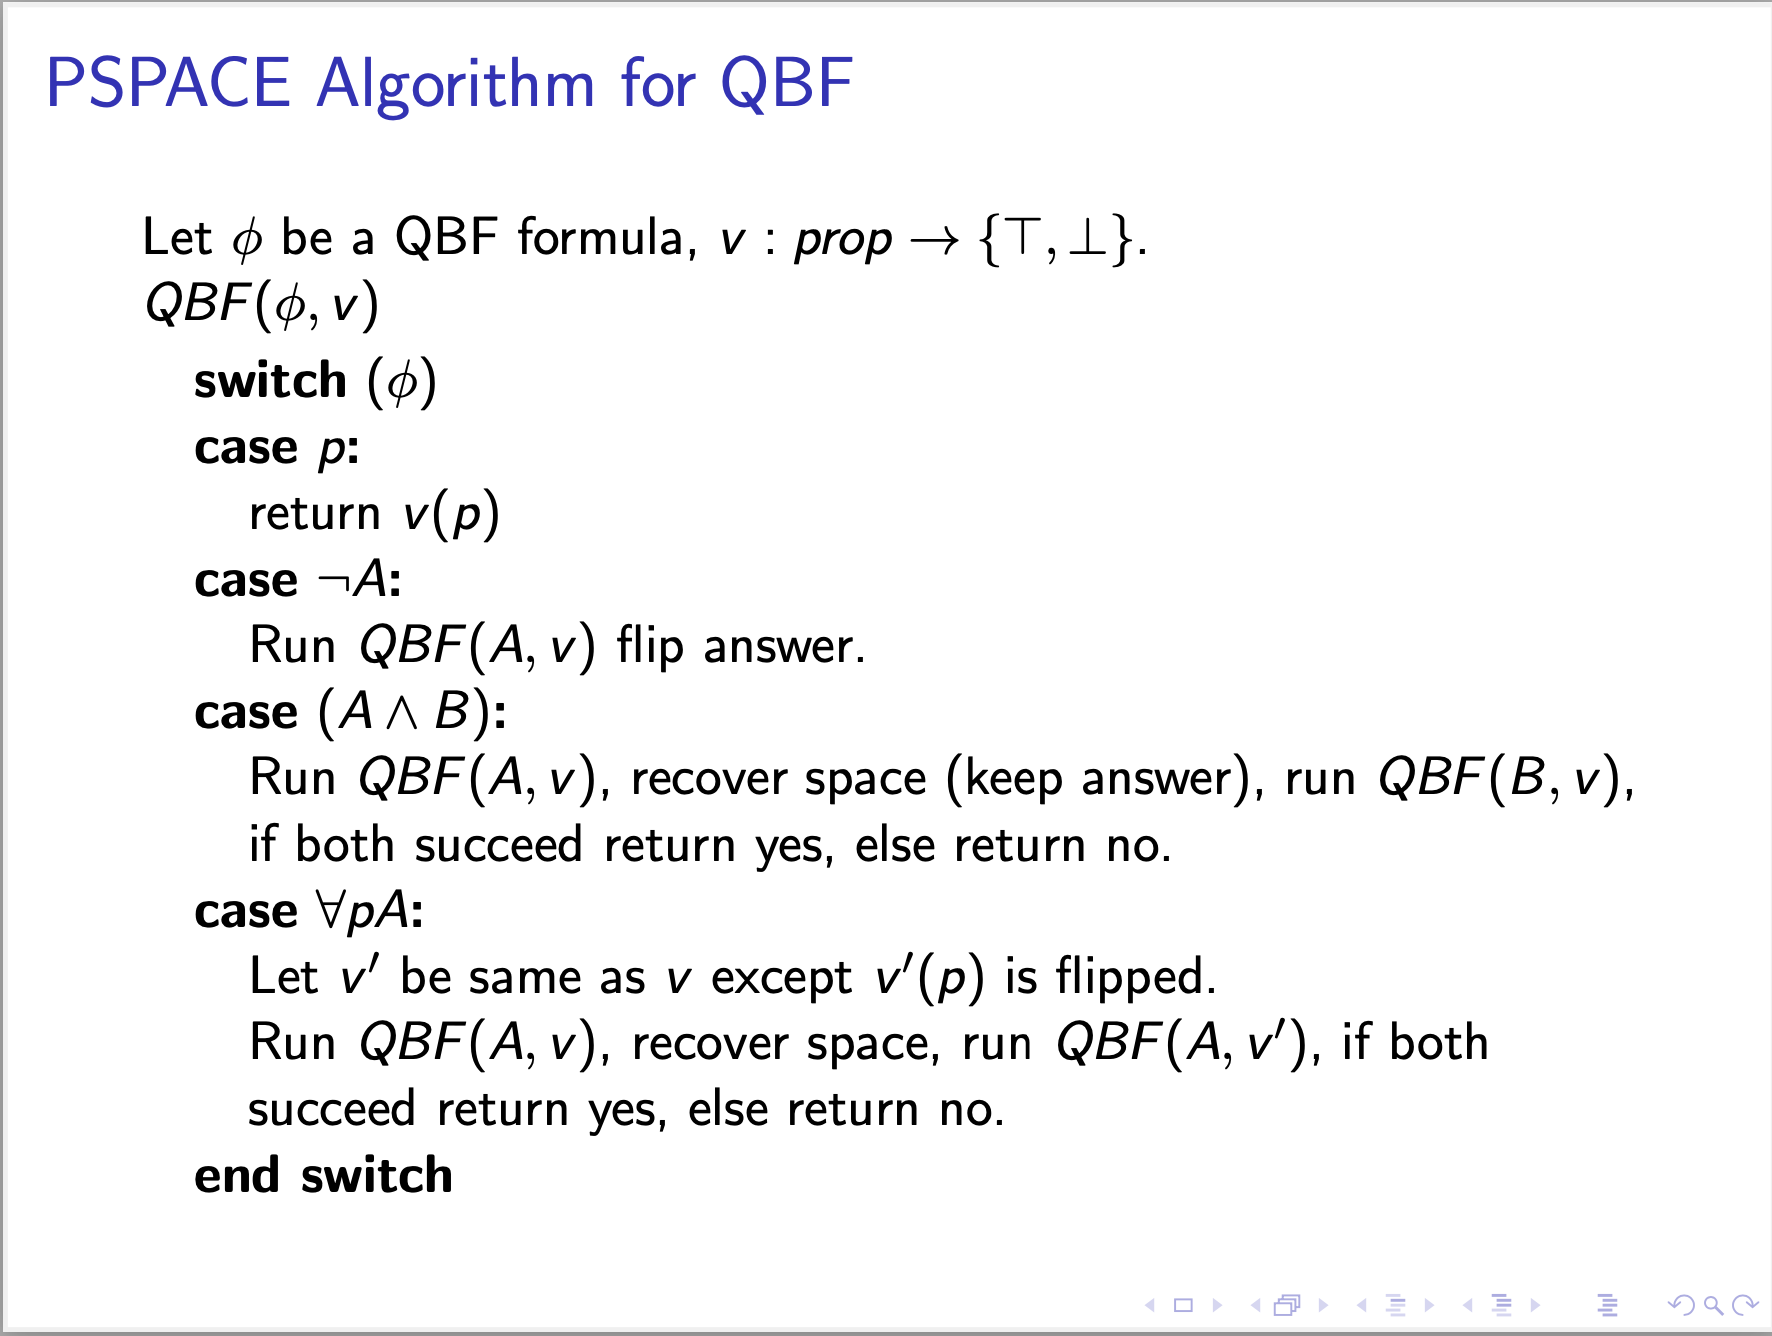
\includegraphics[width=0.8\textwidth]{imgs/QBF-PSPACE.png}}
  \caption{$\pmb{PSPACE}$ Algorithm for QBF in COMP0017 slides}
  \label{fig:QBF-PSPACE}
\end{figure}

With reference to Figure \ref{fig:QBF-PSPACE} above, we prove this recursive algorithm only uses polynomial space.

Let $n$ be the input QBF formula length.

First, with regards to the recursive algorithm's stack depth, it is bounded by the number of operators (i.e. $\land, \lor, \lnot, \exists, \forall$) within the formula. Surely, the number of operators shall not exceed the total character length $n$ of the formula.

For each stack frame, we run at most one $QBF(\phi, v)$ instance at the same time (and clean up its space usage afterwards). Each $QBF()$ instance needs to preserve the temporary state of $(\phi_T, v_T)$. Similarly, temporary formula $\phi_T$ would not exceed the length of the original QBF formula, hence bounded by $n$. Meanwhile, the evaluation mapping $v_T$'s space would not exceed the number of propositions in the formula. The number of propositions would also be bounded by the total character count $n$. Thus we conclude that each stack frame's space usage is bounded by $O(n)$.

The total space usage is bounded by stack depth times each stack frame's space usage, bounded by $O(n \times n) = O(n^2)$. This is within polynomial space hence $QBF \in PSPACE$.

\end{document}